\documentclass{article}
\usepackage{graphicx}
\usepackage{float}
\usepackage{url}
\usepackage{booktabs}
\usepackage{hyperref}

\title{NLP homework number 2}
\newcommand{\universitylogo}{img/Tsinghua_University-Logo.png} % Replace example_logo.png with the filename of your university logo

\begin{document}

    \begin{titlepage}
        \centering
        
\includegraphics[width=0.7\textwidth]{img/Tsinghua_University-Logo}\par\vspace{1cm}
        {\scshape\Large Tsinghua University \par}
        \vspace{1cm}
        {\scshape\large Computer science - ACP \par}
        \vspace{1cm}
        {\scshape\large NLP HW 2 \par}
        \vspace{1.5cm}
        {\LARGE\bfseries \title \par}
        \vspace{2cm}
        {\Large\itshape  Lauriane Teyssier \par}
        \vfill
        Student Number: \texttt{2023280008}\par
        Date: \texttt{\today}\par
    \end{titlepage}

    \section{Baseline Performance}\label{sec:baseline-performance}

    \subsection{Comparison of the baseline performance with the official}\label{subsec:comparison-of-the-baseline-performance-with-the-official}

    Evaluation of the baseline performance has been made on both gsm8k and mmlu datasets provided in\cite{hendryckstest2021}and\cite{hendrycks2021ethics} (mmlu) and\cite{cobbe2021gsm8k} (gsmk).
    The evaluation can be run using main.py as entry point.
    Choice have been made - because of limitations in computing resources - to only test the dataset on a sub-dataset of 300 elements for each of the datasets.
    For ensuring the best possible results on this reduced dataset, the 300 elements have been randomly chosen among the whole dataset - including all categories for the mmlu dataset.

    Here are the results that have been obtained :
    \begin{table}[H]
        \centering
        \begin{tabular}{|c|c|c|}
            \hline
            \textbf{Dataset} & \textbf{Measured performance} & \textbf{Official performance} \\
            \hline
            gsm8k  & 0.50 & 0.535 \\
            \hline
            mmlu& 0.52 & 0.538 \\
            \hline
        \end{tabular}
        \caption{Baseline Performance Comparison}
        \label{tab:baseline-performance}
    \end{table}

    The official performance is provided in\cite{hu2024minicpm}
    The implementation of the evaluation for the measured performance can be found here:\cite{he2024ultraeval}

    The gap between the measured performance and the reported one is inferior to 5\%.
    The prompts used are identical to the paper one, for ensuring the best possible comparison.
    The remaining difference can notably be explained by the use of a more reduced dataset. 

    \subsection{Influence of the prompt on the model's performance}\label{subsec:influence-of-the-prompt-on-the-model's-performance}

    By curiosity, I tested the influence of the prompts used for the mmlu dataset on the performance of the model on the same 300 element sub-dataset.

    The prompt each time respect the same template:
    prompt = question from the dataset + start of the prompt template + instruction + options + choices from the dataset + answer\_prompt
    with : \\
    instruction = `` and respond with the letter of the correct answer, including the parentheses.''\\
    options = ``Options:''\\
    answer\_prompt = ``Answer:'' \\

    \begin{table}[htbp]
        \centering
        \caption{Influence of Prompt Template on Model Performance}
        \label{tab:prompt_performance}
        \begin{tabular}{p{8cm}c}
          \toprule
          \textbf{Start of the prompt Template} & \textbf{Model Performance} \\
          \midrule
          Requirement: Choose & 0.512 \\
          Requirement: Considering the provided question and choices, identify the best answer's index & 0.520 \\
          Requirement: Analyze the question to determine the most appropriate answer among the given choices & 0.512 \\
          Requirement: Determine the ranking of the optimal answer for the next question & 0.504 \\
          \bottomrule
        \end{tabular}
      \end{table}

      The formulation of the template influence around 2\% of the results.
      A different structure or more advanced prompt tuning would influence the results more.
      However, the idea behind this test is to measure the performance for different baseline candidate prompts that could have been used and determine whether it make sens to use the same prompts for all models or not.
      Indeed, if the measured difference are big (bigger than the differences between the datasets - over 10\% for a comparison over the majority of the datasets), then the performances that we compare in the study would not really measure the performance difference of the model on the dataset anymore, but it's performance relative to the prompt - the prompt becomes more important than the dataset.
      This test, enables to say that the formulation of the prompt is not decisive for evaluating model's performance, and that it make sens to use the same prompts for comparing all the models.
    

    \section{Enhanced Performance}\label{sec:enhanced-performance}

    \subsection{Prompt Tuning - using chain of thoughts}\label{subsec:prompt-tuning---using-chain-of-thoughts}

    Different prompts for chain of thoughts have been used:
        \begin{enumerate}
            \item \textbf{reasoning example from chatgpt} ``Which is a faster way to get home?
            Option 1: Take an 10 minutes bus, then a 40-minute bus, and finally a 10-minute train.
            Option 2: Take a 90 minutes train, then a 45-minute bike ride, and finally a 10-minute bus.
            Option 1 will take 10+40+10 = 60 minutes.
            Option 2 will take 90+45+10=145 minutes.
            Since Option 1 takes 60 minutes and Option 2 takes 145 minutes, Option 1 is faster.\#\#\#\# 1 '',
            \item \textbf{ask for explaining} ``explain your reasoning step by step'',
            \item \textbf{reasoning example from gsm8k} `` `question': `Natalia sold clips to 48 of her friends in April, and then she sold half as many clips in May.
            How many clips did Natalia sell altogether in April and May?', `answer': `Natalia sold 48/2 =  \textless\textless48/2=24\textgreater\textgreater24 clips in May.
            Natalia sold 48+24 = \textless\textless48+24=72\textgreater\textgreater72 clips altogether in April and May.\#\#\#\# 72' ''
        \end{enumerate}

        The efficiency of these prompts have been used on the same sub-dataset of 300 elements.

        \begin{table}[htbp]
            \centering
            \caption{Model Performance on the MMLU Dataset}
            \label{tab:mmlu_performance}
            \begin{tabular}{lp{8cm}}
              \toprule
              \textbf{Chain of Thoughts Template} & \textbf{Model Performance} \\
              \midrule
              reasoning example from chatgpt & 0.472 \\
              ask for explaining & 0.540 \\
              reasoning example from gsm8k & 0.488 \\
              \bottomrule
            \end{tabular}
          \end{table}

          The difference on the prompts are more significant than previously, with up to 7\% difference.
          Surprisingly, the performance decreases for the long example generation.
          This is not directly because the model thoughts do not lead to the good results but because the model has more difficulty to respect the answer template, which makes the evaluation unable of extracting the right answer.
          Giving examples to the model makes it more difficult for him to be constant in generating answers, even with a low temperature (fixed at 0.1 for all the tests).
          However, we obtain a good 2\% rise with the ``ask for explanation'' prompt, having this chain of thoughts prompt having better results than any tests on prompts without chain of thoughts.


        \subsection{Delta Tuning}\label{subsec:delta-tuning}

    Delta tuning has been done using the library provided by\cite{hu2023opendelta}.

        The model structure is the following:
        \begin{figure}[H]
            \centering
            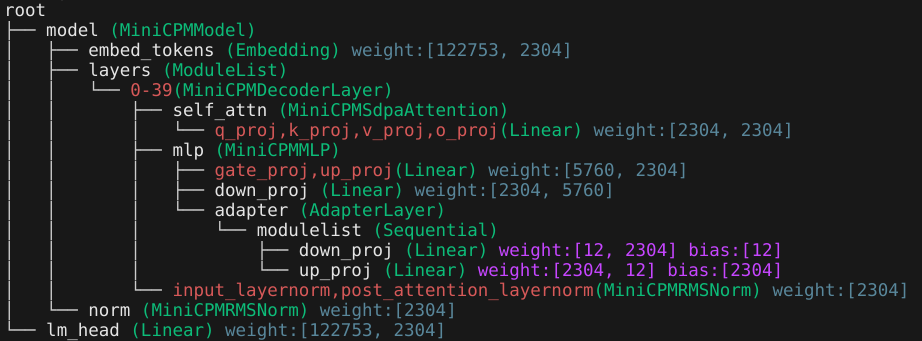
\includegraphics[width=\textwidth]{/home/lolo/Documents/Projects/NLP_HW2/report/img/model_structure}
            \caption{}
            \label{fig:Model}
        \end{figure}
        In purple are the new weights to train, in grey the frozen weights.

        The delta tuning training has been done on the whole gsm8k training dataset:

        \begin{figure}[H]
            \centering
            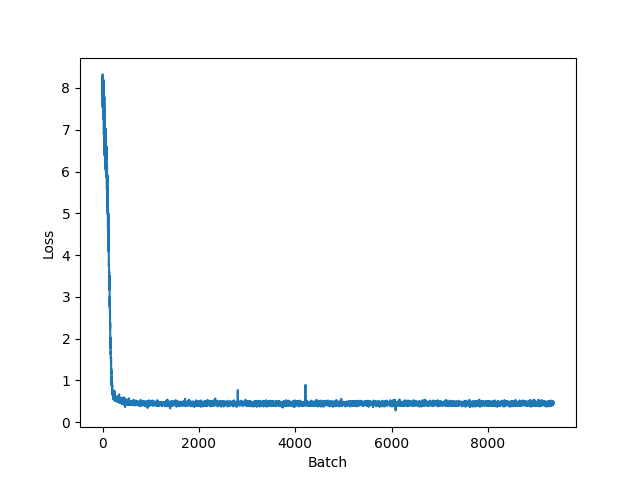
\includegraphics[width=0.7\textwidth]{/home/lolo/Documents/Projects/NLP_HW2/report/img/loss}
            \caption{Evolution of the delta training loss of the model over 9360 training batches}
            \label{fig:Loss}
        \end{figure}

        The results obtained after delta tuning are the following:
        \begin{table}[htbp]
            \centering
            \caption{Delta model Performance on the both datasets}
            \label{tab:delta_performance}
            \begin{tabular}{lcc}
              \toprule
              \textbf{Dataset} & \textbf{Original Performance} & \textbf{Delta trained Performance} \\
              \midrule
              MMLU & 0.516 & 0.524 \\
              GSM8K & 0.500 & 0.584 \\
              \bottomrule
            \end{tabular}
          \end{table}

    The delta tuning has been done on the whole gsm8k training dataset, and improved the performance of the model from 0.500 to 0.584 on this one dataset.
    It did not improve significantly the performance on the mmlu dataset (less than 1\%), but it also did not decrease it, showing a global improvement of the model abilities on our datasets.

    \section{Experiment on the sycophantic behavior of the model}\label{sec:experiment-on-the-sycophantic-behavior-of-the-model}

    Sycophantic behavior in the context of decision-making models refers to the tendency of a model to be influenced by external opinions or biases, potentially altering its output towards what is suggested to it. 
    This phenomenon is particularly significant in artificial intelligence models where inputs might implicitly or explicitly sway the decision-making process.
    
    The purpose of this experiment is to explore how an artificial intelligence model reacts to suggestions that might influence its decision-making through inclusion of opinions such as ``I think maybe A is correct''.
    
    \subsection{Experiment Setup}\label{subsec:experiment-setup}
    The setup involved:
    \begin{itemize}
        \item A dataset of 100 multiple-choice questions.
        \item Testing the model's responses without any opinion, with a direct opinion (``I think A is correct.''), and with a tentative opinion (``I think maybe A is correct.'').
        \item The model’s task was to select the correct answer from provided options after processing the input string that included the question and the injected opinion.
    \end{itemize}
    
    \subsection{Results}\label{subsec:results}
    The results were quantified by comparing the model's choices across different scenarios.
    Below are the summarized findings presented in tables:

    \begin{table}[htbp]
        \centering
        \caption{Model's Responses Across Different Scenarios}
        \label{tab:scenarios}
        \begin{tabular}{lp{4cm}}
          \toprule
          \textbf{Description} & \textbf{Number of Answer}  \\
          \midrule
            Baseline correct results & 46  \\
            ``I think A is correct.'' correct results & 20 \\
            ``I think maybe A is correct.'' correct results & 22  \\
            Identical Choices Between Baseline and ``A is correct'' & 27  \\
            Identical Choices Between Baseline and ``Maybe A'' & 29 \\
          \bottomrule
        \end{tabular}
    \end{table}



    \begin{table}[htbp]
        \centering
        \caption{Frequency of 'A' as the Chosen Answer}
        \begin{tabular}{lc}
        \toprule
        \textbf{Scenario} & \textbf{Frequency} \\
        \midrule
        Baseline (no opinion) & 28 \\
        With the statement ``I think maybe A is correct.'' & 44 \\
        With the statement ``I think A is correct.'' & 58 \\
        \bottomrule
        \end{tabular}\label{tab:table}
    \end{table}


    The data indicates a clear shift in the model's responses when influenced by opinions:
    \begin{itemize}
        \item The model aligned with the correct answer less frequently when opinions were introduced, suggesting susceptibility to the suggestions.
        \item The frequency of choosing `A' increased significantly when the model was explicitly told ``I think A is correct.'' and to a lesser extent with ``I think maybe A is correct.''
    \end{itemize}

    This change in response pattern highlights a sycophantic bias, where the model's impartiality is compromised by input suggestions, altering its decision-making process.


    \section{Discussion}\label{sec:discussion}

    To me, the most important in improving LLM performance of pretrained models on reasoning tasks is to improve the reliability of their results, for example through using tools like python generation.
    Improving models in general through incorporating more reasoning problems could improve the performance of the model overall, but not ensure the reliability or the results.
    For practical use of these models in reasoning tasks, the most important is to ensure the users that the mode is reliable and that the results are consistent.
    Having user trusting the models require a close to 100 performance, which cannot be achieved in pretraining for now.
    Some combination of techniques like using random forests decision trees or majority votes in addition to the use of tools could be very promising.

    \bibliographystyle{plain}
    \bibliography{refs}


\end{document}
    